\documentclass{article}
\usepackage[utf8]{inputenc}
\usepackage{listings}
\usepackage{multimedia} % to embed movies in the PDF file
\usepackage{graphicx}
\usepackage{comment}
\usepackage[english]{babel}
\usepackage{amsmath}
\usepackage{amsfonts}
\usepackage{wrapfig}
\usepackage{multirow}
\usepackage{verbatim}
\usepackage{float}
\usepackage{cancel}
\usepackage{caption}
\usepackage{subcaption}
\usepackage{mathdots}
\usepackage{/home/cade/Homework/latex-defs}
\usepackage{/home/cade/Homework/jlcode}


\title{AMATH 586 Homework 4}
\author{Cade Ballew \#2120804}
\date{May 20, 2022}

\begin{document}
	
\maketitle
	
\section{Problem 1}
Consider the following heat equation with ``linked'' boundary conditions
\begin{align*}
	\begin{cases}
		u_t = \frac 1 2 u_{xx}\\
		u(0,t) = s u(1,t)\\
		u_x(0,t) = u_x(1,t),\\
		u(x,0) = \eta(x),
	\end{cases}
\end{align*}
where $s \neq -1$.   The MOL discretization with the standard second-order stencil can be written as
\begin{align*}
	U'(t) = -\frac{1}{2h^2} A U(t) + \begin{pmatrix} \frac{U_0(t)}{2h^2} \\ 0 \\ \vdots \\ 0 \\ \frac{U_{m+1}(t)}{2h^2} \end{pmatrix}, \quad A = \begin{pmatrix}
		2  & -1\\
		-1 & 2 & -1 \\
		& -1 & 2 & -1\\
		&& \ddots & \ddots & \ddots \\
		&&& -1 & 2 \end{pmatrix}.
\end{align*}
If we enforce the boundary conditions via $U_0(t) = s U_{m+1}(t)$ and suppose that
\begin{align*}
	\frac{U_{1}(t) - U_0(t)}{h} = \frac{U_{m+1}(t) - U_m(t)}{h},
\end{align*}
we find that 
\[
\frac{U_{1}(t) - sU_{m+1}(t)}{h} = \frac{U_{m+1}(t) - U_m(t)}{h},
\]
so
\[
(1+s)U_{m+1}(t)=U_1(t)+U_m(t),
\]
meaning that 
\begin{align*}
U_{m+1}(t)=\frac{1}{1+s}U_1(t)+\frac{1}{1+s}U_m(t),\\
U_{0}(t)=\frac{s}{1+s}U_1(t)+\frac{s}{1+s}U_m(t).
\end{align*}
Then, we have from the MOL discretization that
\begin{align*}
U_1'(t)&=-\frac{1}{2h^2}(2U_1(t)-U_2(t))+\frac{1}{2h^2}\left(\frac{s}{1+s}U_1(t)+\frac{s}{1+s}U_m(t)\right)\\&=\frac{1}{2h^2}\left(\left(-2+\frac{s}{1+s}\right)U_1(t)+U_2(t)+\frac{s}{1+s}U_m(t)\right).
\end{align*}
For $j=2,\ldots,m$, 
\begin{align*}
U'_j(t)=-\frac{1}{2h^2}(-U_{j-1}(t)+2U_j(t)-U_{j+1}(t))=\frac{1}{2h^2}(U_{j-1}(t)-2U_j(t)+U_{j+1}(t)).
\end{align*}
Finally, 
\begin{align*}
U'_m(t)&=-\frac{1}{2h^2}(-U_{m-1}(t)+2U_m(t))+\frac{1}{2h^2}\left(\frac{1}{1+s}U_1(t)+\frac{1}{1+s}U_m(t)\right)\\&=
\frac{1}{2h^2}\left(\frac{1}{1+s}U_1(t)+U_{m-1}(t)+\left(-2+\frac{1}{1+s}\right)U_m(t)\right).
\end{align*}
Putting this back into matrix form, we find that 
\[
U'(t) = \frac{1}{2h^2} B U(t)
\]
where
\begin{align*}
B = \begin{pmatrix}
		-2 + \frac{s}{1 + s} & 1 &&&& \frac{s}{1 + s}\\
		1 & -2 & 1 \\
		& 1 & -2 & 1 & \\
		&&\ddots & \ddots & \ddots \\
		&&&1 & -2 & 1 \\
		\frac{1}{1+s} &&&& 1 & -2 + \frac{1}{1+s} \end{pmatrix}.
\end{align*}

\section{Problem 2}
Applying backward Euler to the system from problem 1, we have the system 
\begin{align}\label{be}
	\left( I - \frac{k}{2h^2}B \right) U^{n+1} =  U^n, \quad U^n = \begin{pmatrix} U_1^n \\ U_2^n \\ \vdots \\U_m^n \end{pmatrix}.
\end{align}
Using Julia, we solve this system with 
\begin{align*}
	\eta(x) = e^{-20(x-1/2)^2},
\end{align*}
$k = h$ and $h = 0.001$ with $s = 2$. We plot the computed solution at times $t = 0.001,0.01,0.1$ as follows. \\
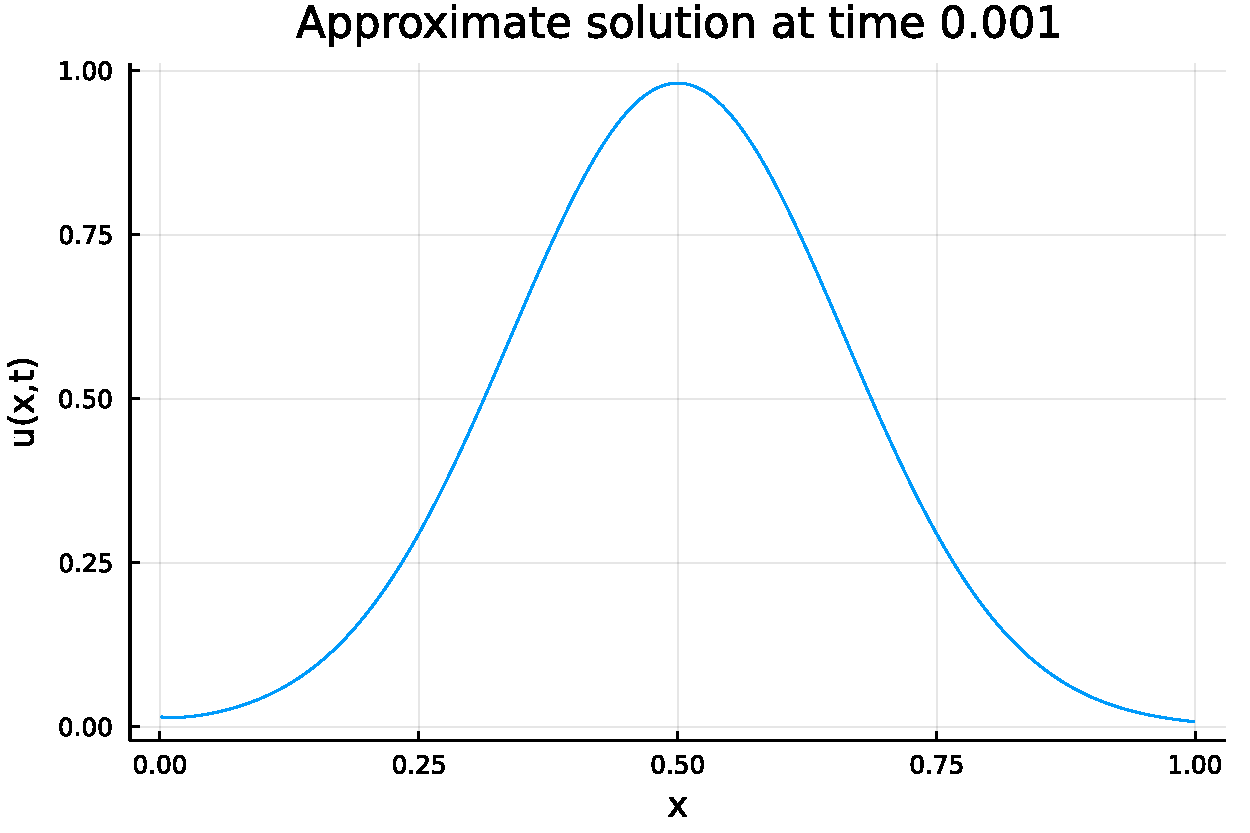
\includegraphics[scale=0.5]{p2_1.pdf}\\
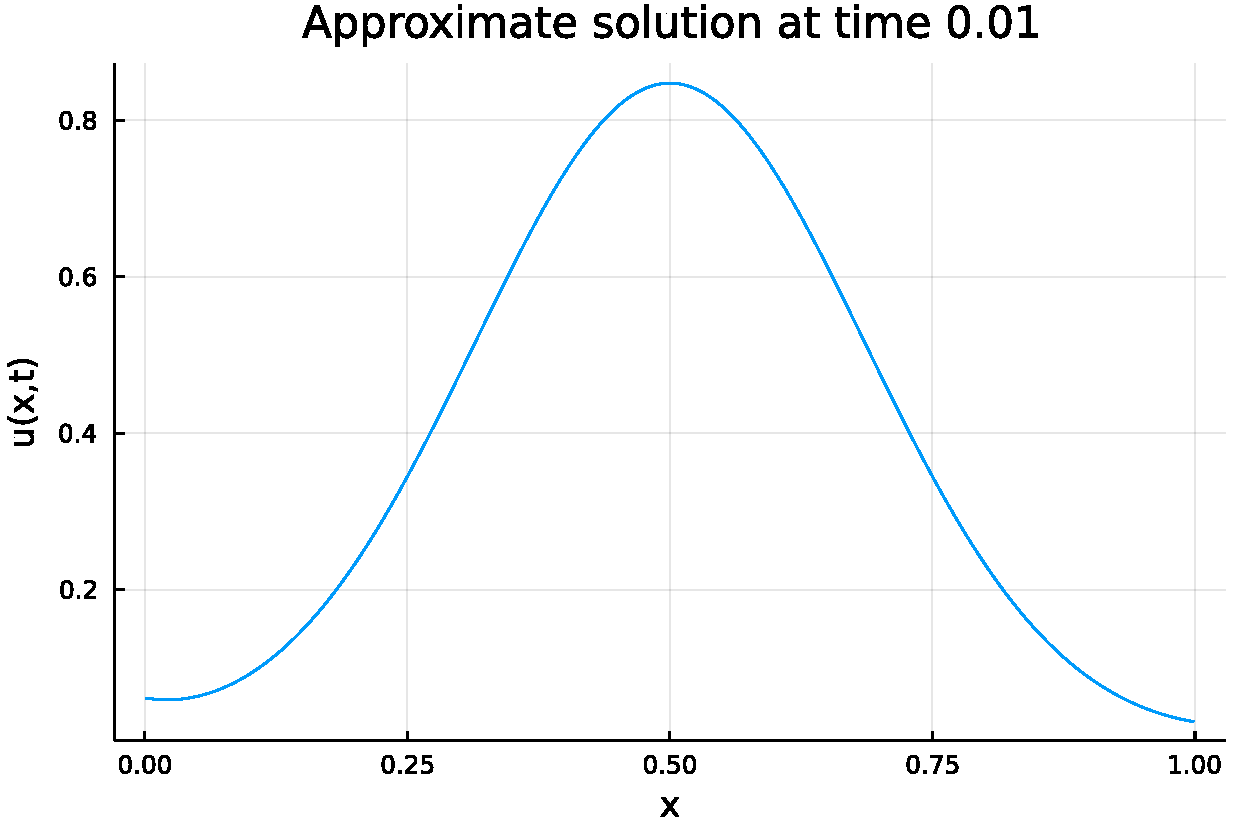
\includegraphics[scale=0.5]{p2_2.pdf}\\
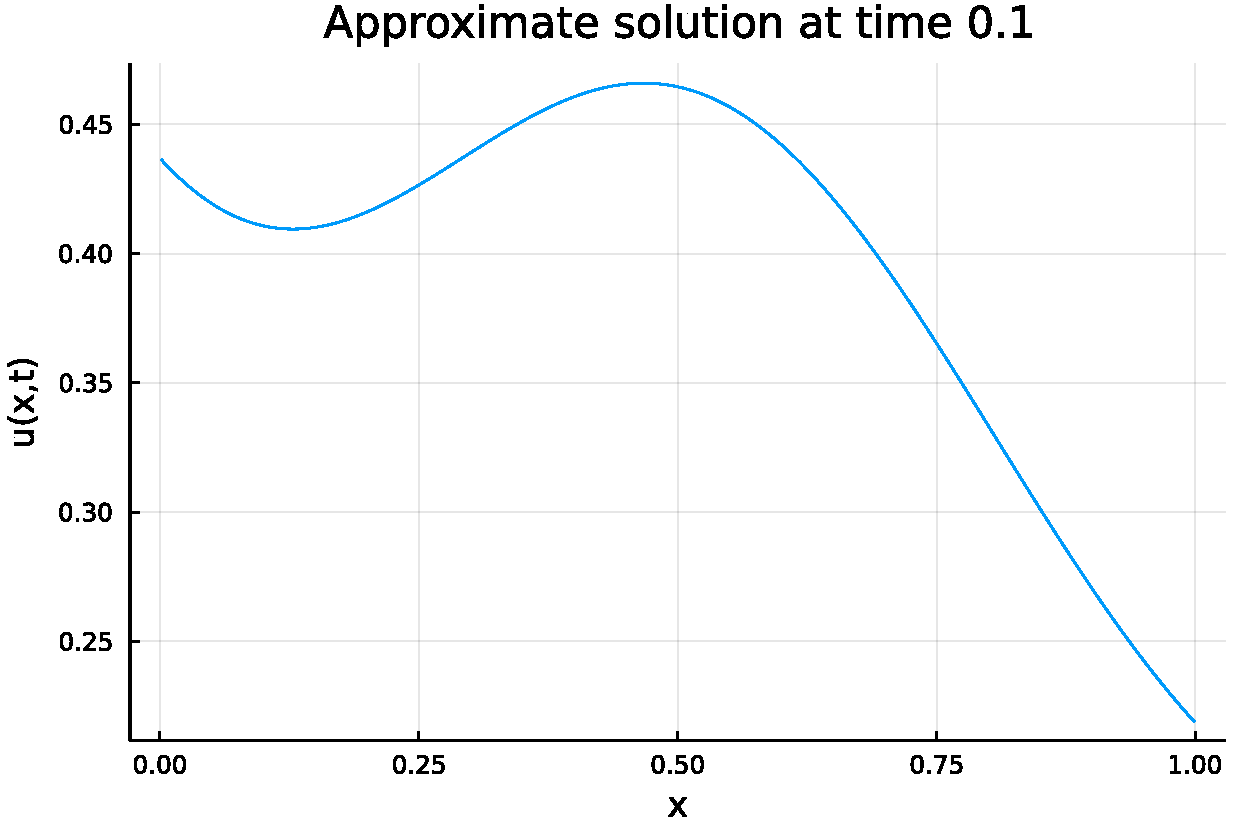
\includegraphics[scale=0.5]{p2_3.pdf}\\
See Appendix A for the Julia code used to do this. 

\section{Problem 3}
Consider the function 
\begin{align*}
	\frac{1}{N} \sum_{j=1}^N \frac{1}{\sqrt{2 \pi t}} \exp \left( - \frac{(x - X_j)^2}{2t} \right), \quad t > 0.
\end{align*}
as an approximation to the density of data points $X_1,X_2,\ldots,X_N,\ldots$ each being a real number arising from a repeated experiment. Using Julia, we generate normally distributed data with $n = 10000$ and plot this function for $t = 0.001,0.01,0.1,1,10$ against the true probabilty density function for the data $\rho(x) = \frac{1}{\sqrt{2 \pi}} e^{-x^2/2}$ in the following plot. \\
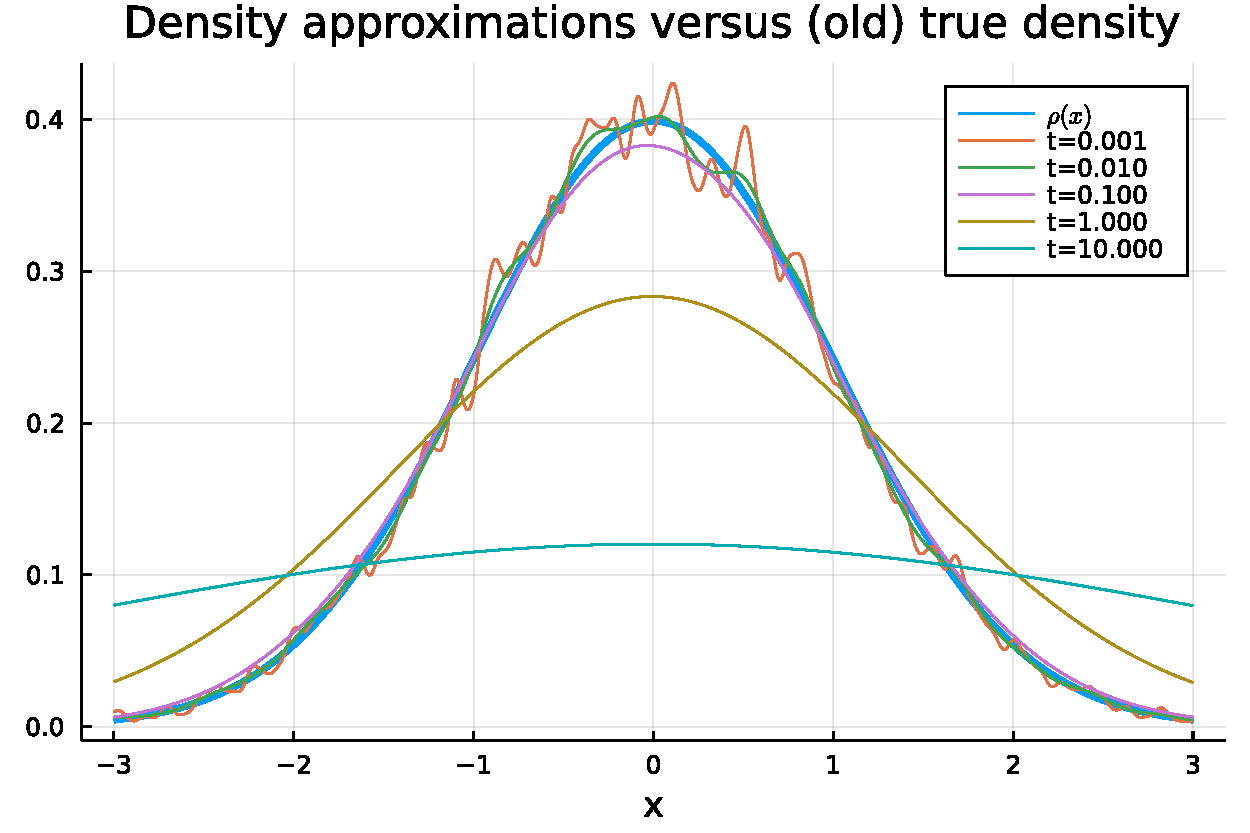
\includegraphics[scale=0.5]{density_approx.pdf}\\
Visually, it seems that $t=0.01$ gives the best approximation to the true density as it is barely visible over the true density. \\
Now, consider data points which instead correspond to the density
\begin{align*}
	\rho(x) = - \frac 2 3 x + \frac 4 3 + \frac 1 2 \sin(2 \pi x).
\end{align*}
Generating data with the provided Julia code, we repeat the experiment and observe the following plot. \\
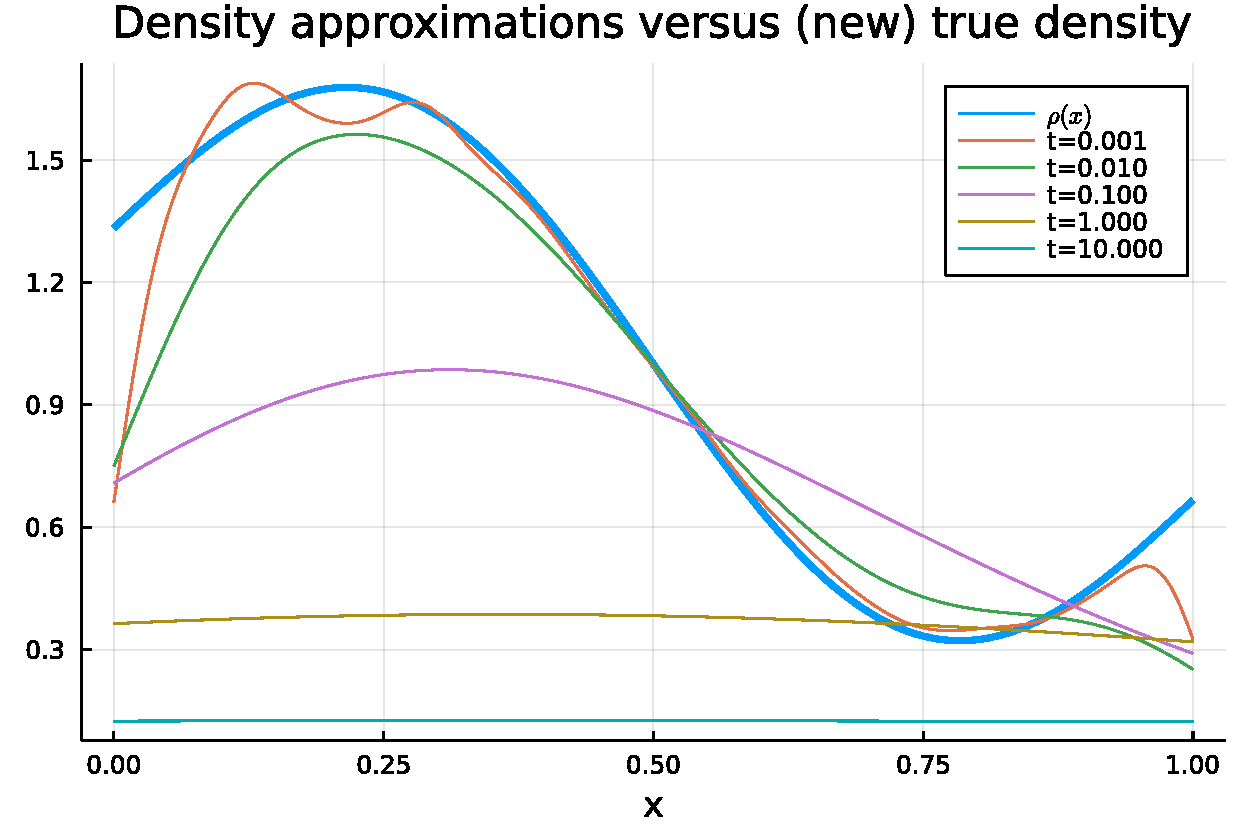
\includegraphics[scale=0.5]{density_approx_new.pdf}\\
Now, $t=0.001$ seems to produce the best approximation. \\
See Appendix A for the relevant Julia code.

\section{Problem 4}
Now, we again generate data $X_1,X_2,\ldots,X_N$ with density 
\begin{align*}
	\rho(x) = - \frac 2 3 x + \frac 4 3 + \frac 1 2 \sin(2 \pi x).
\end{align*}
using the provided Julia code and find $Y_i$ so that $Y_i$ is the number of data points $X_j$ that lie in the interval $[ih,(i+1)h) = [x_i,x_{i+1})$. We then set $U_i^0 = \frac{Y_i}{h N}$ to be the initial condition in the heat equation described in problem 1. We take $N = m$, $h = 0.0001$, $k = 10h$, $s = 2$ and use the Julia code from problem 2 to solve this system. The following plots the computed solution at $t = 0.001,0.01,0.1$ against the true density $\rho$. \\
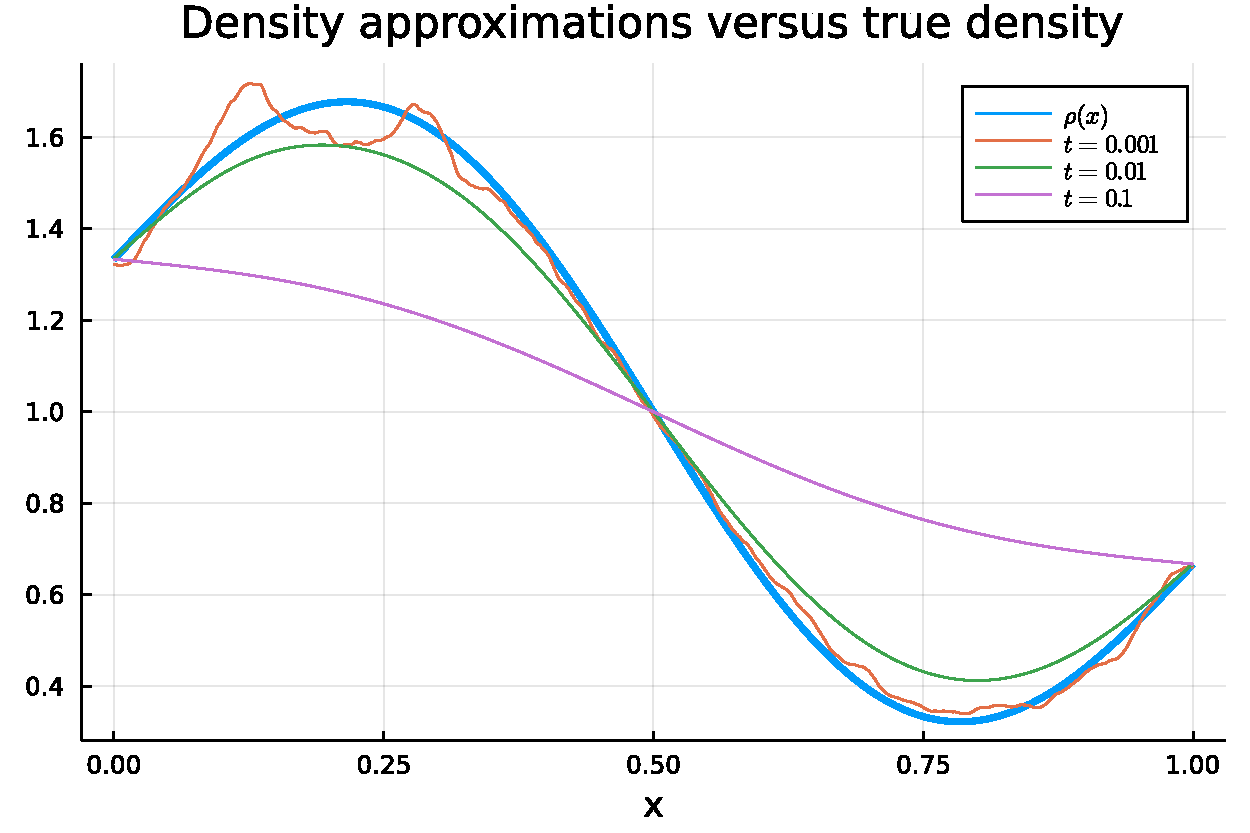
\includegraphics[scale=0.5]{p4.pdf}\\
The result looks quite similar to that of part 2 of problem 3 but does appear slightly better graphically specifically near $x=1$. \\
See Appendix A for the relevant Julia code.

\section{Problem 5}
Let $A=I - \frac{k}{2h^2}B$ where $B$ is defined in accordance with problem 1 and take $s>0$. First, observe that
\begin{align*}
	\left(\begin{pmatrix} 1 & 1 & \cdots & 1 \end{pmatrix} B\right)_1=-2+\frac{s}{1+s}+1+\frac{1}{1+s}=-1+\frac{s+1}{1+s}=0,
\end{align*}
\begin{align*}
\left(\begin{pmatrix} 1 & 1 & \cdots & 1 \end{pmatrix} B\right)_m=\frac{s}{1+s}+1-2+\frac{1}{1+s}=\frac{s+1}{1+s}-1=0,
\end{align*}
and 
\begin{align*}
\left(\begin{pmatrix} 1 & 1 & \cdots & 1 \end{pmatrix} B\right)_j=1-2+1=0
\end{align*}
for $j=2,\ldots,m-1$. Thus,
\[
\begin{pmatrix} 1 & 1 & \cdots & 1 \end{pmatrix} B=0.
\]
This implies that 
\[
\begin{pmatrix} 1 & 1 & \cdots & 1 \end{pmatrix} A=\begin{pmatrix} 1 & 1 & \cdots & 1 \end{pmatrix}I-\frac{k}{2h^2}\begin{pmatrix} 1 & 1 & \cdots & 1 \end{pmatrix}B=\begin{pmatrix} 1 & 1 & \cdots & 1 \end{pmatrix}.
\]
Using the fact that $AU^{n+1}=U^n$ for $n=0,1,\ldots$ inductively, we have that $A^nU^n=U^0$. We now have that
\begin{align*}
	\begin{pmatrix} 1 & 1 & \cdots & 1 \end{pmatrix} A^n&=\left(\begin{pmatrix} 1 & 1 & \cdots & 1 \end{pmatrix}A\right)A^{n-1}\\&=
	\begin{pmatrix} 1 & 1 & \cdots & 1 \end{pmatrix} A^{n-1}=\ldots=\begin{pmatrix} 1 & 1 & \cdots & 1 \end{pmatrix},
\end{align*}
so we can left multiply both sides of $A^nU^n=U^0$ by $\begin{pmatrix} 1 & 1 & \cdots & 1 \end{pmatrix}$ to find that 
\begin{align*}
	&\text{LHS}=\begin{pmatrix} 1 & 1 & \cdots & 1 \end{pmatrix}A^nU^n = \begin{pmatrix} 1 & 1 & \cdots & 1 \end{pmatrix}U^n=\sum_j U_j^n,\\
	&\text{RHS}=\begin{pmatrix} 1 & 1 & \cdots & 1 \end{pmatrix}U^0=\sum_j U_j^0,
\end{align*}
so we can conclude that
\[
\sum_j U_j^n = \sum_j U_j^0
\]
for all $n=0,1,\ldots$. \\
Now, we assume that for $s > 0$, if $y$ is a vector with non-negative entries and $\left( I - \frac{k}{2h^2}B \right) x = y$ then $x$ has non-negative entries. This also means that if $y$ is a vector with non-positive entries and $\left( I - \frac{k}{2h^2}B \right) x = y$, then $x$ has non-positive entries as then $-x$ would have nonnegative entries, so $-y=\left( I - \frac{k}{2h^2}B \right) (-x)$ would have non-negative entries. This of course means that the same property holds for $A^kx=y$. Now, note that any vector $u$ can be decomposed as $u=p+n$ where
\[
p_j=\begin{cases}
	u_j,  &u_j>0\\
	0,  &u_j\leq0,
\end{cases}
\]
\[
n_j=\begin{cases}
	0,  &u_j>0\\
	u_j,  &u_j\leq0,
\end{cases}
\]
for all $j$. Then, by definition,
\begin{align*}
\|A^k\|=\max_{\|u\|_1=1}\|A^ku\|_1.
\end{align*}
If we consider an arbitrary $u\in\real^{m}$ and decompose it as $u=p+n$, then by the triangle inequality and our assumed property of $A$, 
\begin{align*}
\|A^ku\|_1&=\|A^k(p+n)\|_1\leq\|A^kp\|_1+\|A^kn\|_1=h\sum_{j=1}^M|(A^kp)_j|+h\sum_{j=1}^M|(A^kn)_j|\\&=
h\sum_{j=1}^M(A^kp)_j-h\sum_{j=1}^M(A^kn)_j=h\sum_{j=1}^M(A^k(p-n))_j
\end{align*}
Now, we use the property that $\sum_j U_j^n = \sum_j U_j^0$ by considering\footnote{Note that we use $U^k$ instead of of $U^n$ to avoid reusing variables.} $U^0=A^k(p-n)$, $U^k=p-n$ which gives us that
\begin{align*}
\|A^ku\|_1&\leq h\sum_{j=1}^M(p-n)_j=h\sum_{j=1}^Mp_j+h\sum_{j=1}^M(-n)_j=h\sum_{j=1}^M|p_j|+h\sum_{j=1}^M|n_j|\\&=h\sum_{j=1}^M|(p+n)_j|=\sum_{j=1}^M|u_j|=\|u\|_1=1
\end{align*}
Because we can do this for any choice of $u$, we actually have that 
\begin{align*}
	\|A^k\|=\max_{\|u\|_1=1}\|A^ku\|_1\leq\max_{\|u\|_1=1}\|u\|_1=1.
\end{align*}
Because we are able to bound our iteration matrix in this way, we can take $C_T=1$ to conclude that the forward Euler iteration is Lax-Richtmyer stable in the $1$-norm.

\section{Problem 6}
Consider the bi-infinite matrix
\begin{align*}
	L = \begin{pmatrix}
		\ddots & \vdots & \vdots & \vdots  & \iddots \\
		\cdots & L_{-1,-1} & L_{-1,0} & L_{-1,1} & \cdots \\
		\cdots & L_{0,-1} & L_{0,0} & L_{0,1} & \cdots \\
		\cdots & L_{1,-1} & L_{1,0} & L_{1,1} & \cdots \\
		\iddots & \vdots & \vdots & \vdots & \ddots
	\end{pmatrix}                
\end{align*}
and suppose the matrix $L$ defines a bounded linear operator on $\ell^2(\mathbb Z)$ via matrix-vector multiplication with
\begin{align*}
	\ell^2(\mathbb Z) \ni V = \begin{pmatrix} \vdots \\ V_{-1} \\ V_0 \\ V_1 \\\vdots \end{pmatrix}.
\end{align*}
Let $e_k$ denote the $k$th unit vector and let $S_\ell$ denote the $\ell$th shift operator. Then, we let $j\in\mathbb{Z}$ and by basic matrix multiplication we see that 
\[
(Le_k)_j=L_{j,k}.
\]
We can also see from the definition of the shift operator that
\[
S_\ell e_k=e_{k+\ell},
\]
so
\[
(LS_\ell e_k)_j=(Le_{k+\ell})_j=L_{j,k+\ell},
\]
and
\[
(S_{-\ell} LS_\ell e_k)_j=(LS_\ell e_k)_{j+\ell}=L_{j+\ell,k+\ell}.
\]
Because the unit vectors form a basis for $\ell^2(\mathbb Z)$, we can decompose any $V\in\ell^2(\mathbb Z)$ into a sum of unit vectors. $LV=S_{-\ell}LS_\ell V$ for any $V\in\ell^2(\mathbb Z)$ if and only if $Le_k=S_{-\ell}LS_\ell e_k$ for every $k\in\mathbb{Z}$. Thus, by definition, $L$ is shift-invariant if and only if
\[
L_{j,k}=L_{j+\ell,k+\ell}
\]
for every $j,k,\ell\in\mathbb{Z}$. However, this is precisely the definition of of a Toeplitz matrix as $L$ is constant along diagonals, so $L_{i,j}=c_{i-j}$ for a sequence $(c_j)_{j=-\infty}^\infty$. Thus, we can conclude that $L$ is shift-invariant iff $L_{i,j}=c_{i-j}$ for a sequence $(c_j)_{j=-\infty}^\infty$.

\section{Problem 7}
In the notation of Problem 2, for $s > 0$, we wish to establish
that if $y$ is a vector with non-negative entries and $\left( I - \frac{k}{2h^2}B \right) x = y$ then $x$ has non-negative entries. We first establish notation by letting $A=I - \frac{k}{2h^2}B$ and $\alpha=\frac{k}{2h^2}$. We do this by way of Farkas' lemma; namely, we wish to show that there does not exist some $z\in\real^m$ such that $A^Tz\geq0$ and $z^Ty<0$ where $y\geq0$ is given and The "$\geq$" symbol means that all components of the vector are nonnegative. If we can show this, then Farkas' lemma implies that there must exist $x\in\real^m$ such that $Ax=y$ and $x\geq0$ for the same given $y$ which is precisely what we wish to show in this problem.\\
To show our new statement, we note that because $y\geq0$, at least one component of $z$ must be strictly negative in order for $z^Ty<0$ to hold. Thus, it suffices to show that $A^Tz$ must be strictly negative in at least one component when $z$ is strictly negative in at least one component. We do this by considering $i$ to be the index at which $z_i$ is minimized; i.e., $z_i\leq z_j$ for all $j=1,\ldots,m$. Of course, we must have that $z_i<0$. We now show that $(A^Tz)_i<0$. \\
First, note that under our notation, we can write
\begin{align*}
	A^T = \begin{pmatrix}
		1+\alpha\left(2 - \frac{s}{1 + s}\right) & -\alpha &&&& -\alpha\frac{1}{1 + s}\\
		-\alpha & 1+2\alpha & -\alpha \\
		& -\alpha & 1+2\alpha & -\alpha & \\
		&&\ddots & \ddots & \ddots \\
		&&&-\alpha & 1+2\alpha & -\alpha \\
		-\alpha\frac{s}{1+s} &&&& -\alpha & 1+\alpha\left(2 - \frac{1}{1+s}\right) \end{pmatrix}.
\end{align*}
First consider the case where $i=1$. Then,
\begin{align*}
(A^Tz)_1&=z_1+\alpha\left(2 - \frac{s}{1 + s}\right)z_1-\alpha z_2-\alpha\frac{1}{1 + s}z_m\\&\leq 
z_1+\alpha\left(2 - \frac{s}{1 + s}\right)z_1-\alpha z_1-\alpha\frac{1}{1 + s}z_1\\&=
z_1+\alpha\left(1-\frac{s+1}{1+s}\right)z_1=z_1<0.
\end{align*}
In the case where $i=m$, 
\begin{align*}
(A^Tz)_m&=-\alpha\frac{s}{1+s}z_1-\alpha z_{m-1} +z_m+\alpha\left(2 - \frac{1}{1+s}\right)z_m\\&\leq
-\alpha\frac{s}{1+s}z_m-\alpha z_{m} +z_m+\alpha\left(2 - \frac{1}{1+s}\right)z_m\\&=
z_m+\alpha\left(1-\frac{s+1}{1+s}\right)=z_m<0.
\end{align*}
Finally, if $i=2,\ldots,m-1$,
\begin{align*}
(A^Tz)_i&=-\alpha z_{i-1}+(1+2\alpha)z_i-\alpha z_{i+1}\leq-\alpha z_{i}+(1+2\alpha)z_i-\alpha z_{i}=z_i<0.
\end{align*}
Thus, no matter which $i=1,\ldots m$ minimizes $z_i$, $(A^Tz)_i<0$. QED.


\section{Appendix A}
The following Julia code is used for Problem 2.
\jlinputlisting{Problem2.jl}
The following Julia code is used for Problem 3.
\jlinputlisting{Problem3.jl}
The following Julia code is used for Problem 4.
\jlinputlisting{Problem4.jl}



\end{document}
